\RequirePackage[l2tabu,orthodox]{nag}

% TODO: decide if one-sided/two-sided
%\documentclass[headsepline,footsepline,footinclude=false,fontsize=11pt,paper=a4,listof=totoc,bibliography=totoc,BCOR=12mm,DIV=12]{scrbook} % two-sided
\documentclass[headsepline,footsepline,footinclude=false,oneside,fontsize=11pt,paper=a4,listof=totoc,bibliography=totoc]{scrbook} % one-sided
\usepackage[backend=biber]{biblatex}
\addbibresource{references.bib}
\usepackage{booktabs}
\usepackage{tikz}
\usetikzlibrary{shapes.geometric,arrows.meta,positioning,fit,calc}
\usepackage{amsmath}
\usepackage{amsfonts}
\usepackage{amssymb}
\usepackage[most]{tcolorbox}
\usepackage{multirow}
\usepackage{siunitx}
\usepackage{tabularx}
\usepackage{threeparttable}
\usetikzlibrary{backgrounds}
\usetikzlibrary{fit}
\usepackage{graphicx}
\usepackage{minted}
\usepackage{xcolor}
\usepackage{listings}
\usepackage{tcolorbox}
\tcbuselibrary{listings, breakable}
\usepackage{colortbl}  % for \cellcolor
\usepackage{makecell}
\usepackage{float}


% TODO: change citation style in settings
\input{settings}


\definecolor{promptbg}{rgb}{0.97,0.97,0.98}
\definecolor{promptborder}{rgb}{0.85,0.85,0.88}
\definecolor{prompttext}{rgb}{0.18,0.20,0.24}        % Dark slate for commands & text
\definecolor{promptkeyword}{rgb}{0.10,0.38,0.72}     % Muted blue for keywords
\definecolor{promptcomment}{rgb}{0.55,0.58,0.62}
\definecolor{c1}{RGB}{41,128,185}
\definecolor{c2}{RGB}{52,152,219}
\definecolor{c3}{RGB}{155,89,182}
\definecolor{c4}{RGB}{142,68,173}
\definecolor{c5}{RGB}{230,126,34}
\definecolor{c6}{RGB}{211,84,0}
\definecolor{hit}{RGB}{39,174,96}
\definecolor{miss}{RGB}{192,57,43}
\definecolor{warn}{RGB}{243,156,18}


% TODO: change thesis information
\newcommand*{\getUniversity}{Technische Universität München}
\newcommand*{\getFaculty}{Department of Informatics}
\newcommand*{\getTitle}{Thesis title}
\newcommand*{\getTitleGer}{Titel der Abschlussarbeit}
\newcommand*{\getAuthor}{Lívia Cavalcanti Bandeira Julião}
\newcommand*{\getDoctype}{ Master's Thesis in Data Engineering and Analytics}
\newcommand*{\getSupervisor}{Prof. Dr. Jana Giceva Makreshanska}
\newcommand*{\getAdvisor}{Fabian Wenz}
\newcommand*{\getSubmissionDate}{Submission date}
\newcommand*{\getSubmissionLocation}{Munich}
\newcommand{\chit}[1]{\cellcolor{hit!30} #1}
\newcommand{\cmiss}[1]{\cellcolor{miss!25} #1}
\newcommand{\cwarn}[1]{\cellcolor{warn!30} #1}

\newtcblisting[auto counter]{lightprompt}[1][]{
  breakable,
  boxrule=0.6pt,
  colback=promptbg,
  colframe=promptborder,
  arc=1.5mm,
  top=1.5mm,
  bottom=1.5mm,
  left=3mm,
  right=3mm,
  listing only,
  listing options={
    language=bash,
    basicstyle=\small\ttfamily\color{prompttext},
    keywordstyle=\color{promptkeyword}\bfseries,
    commentstyle=\color{promptcomment}\itshape,
    stringstyle=\color{prompttext},       % Overrides default green strings
    identifierstyle=\color{prompttext},   % Ensures standard prompt text stays dark
    showstringspaces=false,
    breaklines=true,
    breakatwhitespace=true
  },
  #1
}

\newtcblisting[auto counter]{lightcpp}[1][]{
  breakable,
  boxrule=0.6pt,
  colback=promptbg,
  colframe=promptborder,
  arc=1.5mm,
  top=1.5mm,
  bottom=1.5mm,
  left=3mm,
  right=3mm,
  listing only,
  listing options={
    language=C++,
    basicstyle=\small\ttfamily\color{prompttext},
    keywordstyle=\color{promptkeyword}\bfseries,
    commentstyle=\color{promptcomment}\itshape,
    stringstyle=\color{prompttext},
    identifierstyle=\color{prompttext},
    showstringspaces=false,
    breaklines=true,
    breakatwhitespace=true,
    tabsize=2
  },
  #1
}

\begin{document}

% Set page numbering to avoid "destination with the same identifier has been already used" warning for cover page.
% (see https://en.wikibooks.org/wiki/LaTeX/Hyperlinks#Problems_with_Links_and_Pages).
\pagenumbering{alph}
\input{pages/cover}

\frontmatter{}

\input{pages/title}
\input{pages/disclaimer}
\input{pages/acknowledgments}
\chapter{\abstractname}

Automated vulnerability patching promises to close the gap between vulnerability discovery and remediation. While Code Property Graphs (CPG) provide rich structural representation for automated discovery, context-aware code patching requires understanding and adherence of the codebase style and logic. 
Some of the current LLM approaches rely on parametric knowledge acquired during training, which previous studies have shown to be insufficient for complex, real-world patching without external structural guidance and retrieved in-context demonstrations\cite{ye2026well, yin2024thinkrepair, gao2023what, shao2026fix}.
However, the effectiveness of retrieval-augmented, agentic LLM pipelines in addressing this limitation, and even to what extent it occurs in modern LLMs, remain underexplored. 

This thesis presents an empirical study of  structure-aware Retrieval-Augmented Generation (RAG) for vulnerability patching. We evaluated an agentic, tool-calling ReAct patch-generation pipeline by comparing unsupervised structural  embeddings against CodeBERT-based semantic embeddings and their hybrid combination.
The architecture was assessed on two main tasks: vulnerability classification via retrieval and patch generation.
Two datasets of different complexity were used to performance evaluation: AutoPatch, a well-curated dataset, and CVEFixes, real-world for different tasks and very rich dataset.
To compare the impact of the LLM backbones, we benchmarked thee models: GPT-5.3-Codex, security specialized model; GPT-4o, a general purpose cheaper model; and an open weights alternative, DeepSeek-V4-Flash.

The results indicate that structure-aware retrieval is a viable but complementary component of automated patching pipelines. Rather than a superior design, its performance depends on the vulnerability class and the downstream model.


\microtypesetup{protrusion=false}
\tableofcontents{}
\microtypesetup{protrusion=true}

\mainmatter{}

\chapter{Introduction}\label{chapter:introduction}

\section{Motivation}

Software vulnerabilities are often variations of flaws that have already been identified, disclosed, and fixed somewhere else.
Once a vulnerability is found and patched in one project, the same bug class routinely resurfaces in other projects that share a library, a coding pattern, or simply a common ancestor in the open-source dependency graph.
Public vulnerability catalogs exist to prevent this knowledge from being lost.
For a given entry, the removed and/or added code marks the fix, and the surrounding, unchanged code marks the vulnerable context in which that fix had to be applied.
Reapplying a known fix to a new, similarly vulnerable codebase is, in principle, a matter of recognizing that context elsewhere and porting an analogous change.

In practice, this recognition step does not scale.
Continuously cross-referencing a project's codebase against a growing catalog of disclosed vulnerabilities is tedious, requires specialized security expertise, and competes with feature work for developers' time.
This is especially burdensome for volunteer-driven open-source projects, where the pace of remediation lags the pace of disclosure.
On top of that, the cost of this lag is asymmetric. 
When a known vulnerability remains unpatched in a downstream project, it can be exploited via a public proof of concept, and the project's adoption and reputation suffer if it is seen as insecure.
%TODO: find a citation quantifying the average time-to-patch for known CVEs in open-source projects (e.g., from an OSS security report) to support this claim with data.
% Or the budgetary impact of vulnerability incidents

\section{Research Background}

To meet compliance requirements, organizations must adhere to international standards and regulations such as ISO/IEC~27001~\cite{iso27001}.
This standard establishes best practices for data protection, cyber-resilience, and operational excellence.
To satisfy it and improve development robustness, enterprises must anticipate and adapt to vulnerabilities and potential attacks.
For software companies, this demands evolving software development life cycles to rapidly identify, generate, and deploy risk mitigations.
One promising approach is to integrate automated systems that proactively generate patches for vulnerable programs.

With the advent and adoption of Large Language Models (LLMs), a new avenue for automated remediation has emerged.
%TODO: restore/verify the Xia_2024 survey citation on LLM-based automated program repair; add its BibTeX entry to references.bib once confirmed.
However, current LLM-based approaches remain insufficient for security patching, for two primary reasons:

\begin{enumerate}
    \item \textbf{Semantic misunderstanding.} 84--94\% of AI-generated patches rely on localized fixes that fail to address root causes, making them significantly more fragile and easier to bypass than human-authored patches~\cite{mahmud2025systematic}.
    \item \textbf{Vulnerability identification failures.} Models may misidentify vulnerability contexts, with some retrieval tasks showing failure rates as high as 91.6\%~\cite{McClanahan2024Meets}.
    This leads to semantic hallucinations, in which a model applies mitigation steps to the wrong operating system~\cite{McClanahan2024Meets} or package version~\cite{zemicheal2024llm}, creating a false sense of security while leaving the actual system exposed.
\end{enumerate}

\section{Problem Statement}

Both failure modes above share a common root cause: the model is not provided with the right context at the right level of abstraction.
Providing lengthy raw source code compounds this problem, since vulnerability-relevant logic is diluted by implementation details and boilerplate, degrading the quality of security analysis.
%TODO: restore/verify the "contextenhancedYang" citation and its "Analysis Focus Drift" terminology; add BibTeX entry once source is confirmed.
Under this effect, which prior work terms Analysis Focus Drift, the model ends up performing a generic code-quality review rather than a targeted vulnerability analysis.
There is, therefore, an opportunity to develop methodologies that concentrate security-relevant information while filtering out implementation noise.

Retrieval-augmented approaches are a natural fit for this gap, as, rather than asking an LLM to reason about a vulnerability from generic pretraining knowledge, they supply it with structurally similar, previously-fixed vulnerabilities as grounding evidence.
Prior work shows that knowledge bases can improve LLM responses in security applications~\cite{Seo2025AutoPatchMF, guo2025bluecodeagentblueteamingagent}.
%TODO: restore/verify the du2025vulrag and wang2025valign citations on knowledge-base-augmented vulnerability repair; add BibTeX entries once confirmed.
However, it remains unclear how retrieval, code representation, and historical context can improve patch quality, particularly in agentic pipelines where retrieval, reasoning, and patch generation are handled by separate components.
This thesis investigates that question by treating each historical fix as a pair of code property graphs: one for the patched code and one for the code before the fix, using the latter as a vulnerability signature that can be indexed, retrieved, and handed to an LLM as targeted context.

\section{Scope and Positioning}

This thesis does not aim to replace security experts or to discover previously unknown vulnerabilities.
The proposed pipeline only works once a vulnerability has been identified and fixed by a developer; therefore, it does not detect zero-days.
Instead, its goal is to maximize the propagation of that human knowledge, to free security experts' time to find genuinely new vulnerabilities, to reduce the window of exposure for already-known ones, and to let teams without dedicated security expertise keep their codebases free of previously cataloged flaws.

% is it really necessary?
Concretely, the system assumes that the vulnerable function to be patched, and its CWE category, are already known and given as input; detecting and localizing a vulnerability are outside the scope of this thesis. The retriever only needs the function's code, not its CWE, to find a structurally similar historical fix. 
What this thesis contributes is (1) retrieving a structurally similar, historically fixed example for that already-characterized vulnerability, and (2) using that example's own metadata (its CWE, CVE identifier, root cause, variable/function mappings, and patched code), together with the target's CWE, to assist patch generation.

%TODO: add a closing paragraph summarizing this thesis's concrete contributions (e.g. CPG-based diff embedding, FAISS/HNSW retrieval, patch-generation and evaluation pipeline) and a one-paragraph roadmap of the remaining chapters (Dataset, Methodology, Evaluation, ...).

% !TeX root = ../main.tex
% Add the above to each chapter to make compiling the PDF easier in some editors.

\chapter{Literature Review}\label{chapter:literature-review}


\section{Patching}
Most vulnerabilities are not entirely novel; the knowledge required to address a new flaw is often already available in previously published fixes for similar issues. Since many software flaws recur across different programs or modules, existing patches can be automatically extracted, adapted, and applied to structurally similar code \cite{Shariffdeen2020}.
This strategy has been explored in Automated Program Repair, and prior work has shown how automated repair systems leverage existing defect and fix-pattern histories to generate patches for newly discovered bugs and vulnerabilities \cite{legoues2019}.

One early way to explore code to find vulnerabilities is to use tools like CodeQL and Joern. Such tools perform static analysis over a graph representation of the code, like encoding control flow, data flow, and syntactic structure to search for known patterns.
Even though these graph-based traversal approaches made vulnerability search much easier and more automated, they require expertise in the language and in the domain-specific vulnerabilities. To scale the search for vulnerabilities and avoid missing one because its pattern was not explicitly searched, it is necessary to shift from hand-crafted rules to an automated search.

\section*{Structural Retrieval and Graph Edit Distance}
Graph edit distance (GED) is defined as the minimum-cost sequence of vertex and edge insertions, deletions, and substitutions required to transform one graph into the other \cite{gao2010survey}.
This classical approach evaluates the structure directly and can be applied to arbitrary graph types, including as a measure of structural similarity between two graphs. This makes them a promising approach for identifying vulnerable structures already known in new code without any language as a proxy, and for reusing the graph knowledge directly in the search.
However, GED is NP-hard; additionally, exact/near-exact computation doesn't scale to corpus-level retrieval over thousands of historical fixes. 

This scalability issue is particularly relevant for security applications.
Feng et al. explore it in the context of vulnerability search, showing that control-flow-graph-based bug search does not scale to firmware corpora due to the cost of graph matching. Their approach converts CFGs into high-level numeric feature vectors that support real-time approximate
search via hashing \cite{feng2016scalable}. 
Xu et al. replace these hand-crafted features with a learned graph neural network embedding for
the same cross-platform bug-search task, reporting large accuracy gains over the hand-engineered baseline \cite{xu2017neural}. 
% the following work is interesting, but i didn't train any of the models so it can be used as a downside
% More generally, SimGNN reframes GED computation itself as a learning problem, training a neural network to approximate GED directly rather than computing it exactly \cite{li2019simgnn}. 
These works exemplify that structural similarity for security-relevant graphs is best operationalized by fixed-length embeddings whose distances approximate structural similarity, enabling standard approximate nearest-neighbor search over large historical corpora.
% (not by computing GED directly at query time, )


\section{Structural and Semantic Code Embedding Techniques}

Traditional graph classification frequently uses non-parametric graph kernels, offering computationally lightweight approaches that can run locally without requiring substantial overhead. 
One of its fields is structural comparison, whose core is the Graph Isomorphism problem, which determines whether the topologies of two graphs are identical. 
While no general polynomial-time algorithm for Graph Isomorphism is currently known \cite{garey1979computers, babai2016graph}, practical upper bounds on the computational complexity of the 1-dimensional Weisfeiler-Lehman (WL) color refinement test have been established \cite{weisfeiler1968reduction}.

The $1$-WL test characterizes graph topology through an iterative color-refinement process. 
At each iteration, a node aggregates its current label with the sorted multiset of its immediate neighbors' labels and hashes the resulting tuple into a new unique label. 
This process repeats until the label distribution between two compared graphs diverges or a fixed cutoff of $k$ iterations is reached; this latter only allows the isomorphism conclusion for the evaluated subgraph. 

The WL Fast Subtree Kernel \cite{shervashidze2011wl} applies this mechanism to a Reproducing Kernel Hilbert Space(RKHS), calculating the inner product of label histograms accumulated over $k$ iterations.
This approach establishes an expressivity benchmark for graph representations. However, despite its computational efficiency, $1$-WL is limited to local neighborhood tree structures defined by iterative local multiset hashing, preventing it from capturing higher-order global substructures such as cycles and cliques. 

The Graph Isomorphism Network (GIN) \cite{xu2019gin}, which bridges graph kernels and deep learning and is designed to maximize the discriminative power of Message-Passing Neural Networks, proved to be as powerful as the Weisfeiler-Lehman graph isomorphism tests. 
To achieve this performance, GIN uses learning neighborhood aggregation via a parameterized function, in which each node embedding iteratively encodes the structure of its k-hop neighborhood. 
To have the same power as 1-WL, GIN requires that both the neighborhood aggregation and graph-level readout functions must be strictly injective. 
A sufficient number of iterations is required to discriminate graphs; 
While deeper iterations are required for larger structural representations, features from early iterations may generalize better depending on the task.
% TODO: put the investigation of the number of iteration as future work

GraphFVD applies the graph embedding principles to the software security context.
It learns graph embeddings from the Code Property Graph code representation
Rather than embedding whole-function graphs, GraphFVD extracts property-graph slices (PrVCs) from the CPG and embeds them using a Hierarchical Attention Graph Convolutional Network.
Their experiments report that this slice-level representation outperforms both function-level and sequence-level slice baselines for vulnerability detection \cite{shao2025graphfvd}. 
This aligns with our design choice to embed a bounded slice rather than the full function CPG.
However, whereas GraphFVD's embeddings feed a supervised classifier for single-function detection, our approach indexes a historical corpus for a retrieval-augmented analysis.
Therefore, the two tasks share a representation, but their task objective diverge.

Complementing local message-passing architectures, the Network Laplacian Spectral Descriptor (NetLSD)\cite{netlsd} provides a global, multi-scale topological representation. 
NetLSD computes a heat-trace signature from the graph Laplacian's eigenvalues, yielding a permutation- and size-invariant embedding that requires no training and is comparable across graphs of different sizes \cite{netlsd}. It captures macro-level structural dynamics without requiring supervised training, making it computationally effective for comparing heterogeneous graph structures.

In contrast to purely structured embeddings, transformer-based models capture lexical and semantic regularities in source code. CodeBERT \cite{feng2020codebert} provides a pre-trained embedding that models token sequences, capturing variable naming conventions, API usage patterns, and control structure semantics—information that remains opaque to purely topological representations.

These embedding strategies of encoding code prioritize different aspects. WL and NetLSD are non-parametric structural descriptors that provide deterministic, invariant topological comparisons without training. GIN, just like GraphFVD, learns structural aggregation for specific vulnerability patterns. CodeBERT captures token-level semantics while lacking structural dependencies. 
Because no single representation captures both fine-grained topological flows and token-level semantics, combining structural graph embeddings with lexical representations offers a promising direction for vulnerability analysis and code retrieval.

\subsection*{Retrieval-Augmented Secure Code Generation}

RESCUE applies retrieval-augmented generation to secure code generation. It uses a hybrid knowledge base that combines vulnerability-fix data distilled into security guidelines with static program slicing to extract security-focused code examples. At retrieval time, RESCUE performs a hierarchical, multi-faceted lookup: first, it identifies the vulnerability type (CWE level) from the task description, then it retrieves fine-grained secure code examples within that type. 
RESCUE targets code generation for known vulnerability classes, while our pipeline targets the repair of already identified vulnerable functions. Both systems share key architectural insights by using program slicing to isolate security-relevant statements before embedding and employing hierarchical retrieval rather than flat nearest-neighbor lookup. Program slicing as a mechanism to concentrate security focus emerges as a convergent design pattern across recent work — alongside GraphFVD's property-graph-based vulnerability candidates and LLMxCPG's CPG-based slicing — reinforcing that isolating security-relevant subgraphs, rather than embedding whole functions, is a broadly validated approach for vulnerability-related tasks.

\section{Agentic Patching Frameworks}

LLM-based program repair has increasingly applied agentic frameworks that allow the model to iteratively gather context, interact with external tools, and revise its own output. (cite)

An example of this approach is AutoPatch, which leverages RAG-DB-assisted prompting to perform vulnerability detection and patching on a benchmark that mixes real-world and augmented Common Vulnerabilities and Exposures (CVEs).
The work evaluated the architecture against five popular LLMs, with GPT-4o achieving the best performance, yielding F1-scores of 90.3\% for vulnerability verification and 94.1\% for patching. The system performs particularly well in concurrency-related issues, validation, and logic handling. Furthermore, AutoPatch demonstrates greater cost efficiency than fine-tuning approaches with 10 epochs, incurring an approximately 1,209\% cost increase, while non-incremental fine-tuning at five CVE intervals resulted in a 5,230\% increase. The AutoPatch built benchmark serves as one of the two primary evaluation datasets utilized in this thesis (see Chapter~\ref{chapter:dataset}).
% To ensure the reliability of the generated patches, AutoPatch employs a rigorous patch-verification feedback loop. After a Code Patcher agent generates a candidate fix, the output is routed back to a Vulnerability Verifier agent. Using previously constructed one-shot examples, the Verifier analyzes the patched code for any remaining vulnerabilities. This cycle iterates until either no vulnerability is detected or a developer-specified maximum number of iterations is reached. While the average loop count was close to 1 across all models, certain difficult cases required more iterations (up to 8 for DeepSeek-R1 and 10 for o3-mini). These findings emphasize that context-aware verification—heavily reliant on in-context examples—is critical for capturing the semantic complexity of real-world vulnerabilities and surfacing logic inconsistencies.

Applying a similar tooling-based architecture, RepairAgent proposes an autonomous agent powered by Large Language Models to dynamically fix software bugs \cite{bouzenia2025repairagent}. 
With AutoPatch, RepairAgent represents a similar agentic generation proposed in this thesis in terms of task framing. 
The introduced agent plans and executes actions through a predefined set of rules that allows the LLM to gather information about the bug, gather repair ingredients, and validate fixes.
To evaluate these patches, the agent automatically applies the fix and executes the project's test suite, using the resulting test feedback to inform subsequent iterations. The agent decides to stop its iterative loop only when a patch successfully passes all validation tests or when a predefined computational budget is exhausted.
They evaluate their approach against Defects4J which contains 835 bugs .
% RepairAgent imposes an average cost of 270,000 tokens per bug, which, under the current pricing of OpenAI’s GPT-3.5 model, translates to 14 cents per bug. An additional evaluation on a set of recent bugs [25] shows that RepairAgent is able to achieve similar performance on single-line bugs while being a bit worse on multi-line and multi-file bugs, mainly, due to a higher complexity of bugs in GitBug-Java dataset.
% We believe from these results that RepairAgent is not much affected by potential data leakage of Defects4J.
% how does it decide when to stop, how does it evaluate patches.
% tool-augmented agentic loop, giving the LLM explicit actions for inspecting the codebase, retrieving relevant
% context, and validating candidate patches, and is the closest prior system to our own agentic generation layer in terms of task framing \cite{bouzenia2025repairagent}
% - ReAct — the general reasoning+acting loop RepairAgent (and your own agentic layer) build on. Cite as the pattern, not as a patching system itself.
% - Self-Refine — iterative self-critique loop; relevant if your agentic generation layer does any revision/retry step. If it doesn't, don't force this citation in — only include what you actually build on.
 
 QLCoder	agentic framework that automatically synthesizes CodeQL queries directly from CVE metadata. It bridges the gap between natural language vulnerability reports and actionable detection tools by embedding an LLM in an iterative synthesis loop that uses execution feedback to verify query correctness.	"RQ1: For how many real-world CVEs can QLCoder successfully generate syntactically valid and semantically precise queries?
 Structured Synthesis Loop: The agent proposes a query, a validator executes it on vulnerable and patched versions of a repository, and feedback is provided to refine the next proposal.
MFix Discrimination: Ensures the synthesized query is precise enough to flag the vulnerable version but remain silent on the patched version."	CWE-Bench-Java: 176 CVEs across 111 Java projects; 42 different CWE categories, such as Path Traversal (48), Cross-Site Scripting (36), and Code Injection (20); 65 CVEs reported in 2025 after Claude Sonnet 4 cutoff

MAAP is a self-evolving, role-specialized multi-agent framework designed for end-to-end automated vulnerability repair (AVR) in Python codebases. It addresses the limitations of single-agent approaches—such as context overload and myopic decision-making—by decomposing vulnerable repositories into fine-grained subtasks	
Contextual-Bandit Router: Learns to assign subtasks to the most appropriate specialized agents to optimize for success, cost, and latency.
% Retrieval-Augmented Knowledge Base: Stores successful and failed repair trajectories (AST diffs and rationales) to guide agents and prune ""dead-end"" explorations.
% Agent Factory: Dynamically spawns new specialized agents when the system encounters novel vulnerability patterns or low success rates"	VAITP selection: 120 real-world Python CVEs(Input validation and sanitization, memory corruption, authentication/session management). AI-generated and human-verified code snippets of vulnerable and patched versions

\chapter{Dataset}\label{chapter:dataset}
\section{Dataset}
% -- keep as-is, but decide: does this need to move before Methodology
% since "AutoPatch dataset" is referenced mid-pipeline? --
% content: AutoPatch dataset (evaluation benchmark)

\subsection{AutoPatch}
The AutoPatch dataset contains high-severity CVEs disclosed in 2024 and 2025 and collected from the GitHub Advisory Database, Openwall [36], and the Chromium issue tracker with a custom crawler.
It includes 57 vulnerabilities from the Linux Kernel and 10 from the Chromium project.
For each CVE, 75 vulnerable and its respective patched code were generated by using 5 LLMs:  Code Llama (13b-instruct), DeepSeek Coder (v2-lite), DeepSeek-R1 (32b), GPT-4o, and OpenAI o3-mini.
The augmentation strategies included  inserting unreachable code fragments, adding random codes in comments, varying whitespace and formatting, defining a useless function, and introducing extraneous newline characters. (copied and paste from the paper)

\subsection{CVEfixes}
% content: CVEfixes dataset (retrieval knowledge base) -- Origin, Collection method, Composition used in this thesis

\chapter{Methodology}\label{chapter:methodology}
\section*{Methodology}

% -- your framing paragraph, minus the graph-edit-distance citation --
% content: "This work proposes a structure-aware RAG framework..." through
% "...identify the lines that introduce security breaches."

\subsection*{Architecture}
% content: KB + agentic framework description, Patcher Agent / Vulnerability Verifier Agent bullets, figure
This project builds a structure-aware retrieval system for vulnerability fixes:

Load vulnerable vs fixed code pairs.
Build a vulnerability-focused graph per pair.
Embed those graphs into vectors.
Index vectors in FAISS.
Retrieve nearest historical fixes for new queries.
Optionally generate patches with an LLM.
Evaluate retrieval and patch quality.


Where each stage lives:
Entry CLI orchestration: main.py
Config and active dataset/embedder selection: config.yaml
Dataset loading and registry: \_\_init\_\_.py
CVEfixes pinned-file dataset variant: cvefixes\_file.py
Split logic (including precomputed splits): split.py
Index build pipeline: indexing.py
FAISS wrapper and metadata persistence: faiss\_index.py
Query batch retrieval: query.py
Retriever search call: retriever.py
Embedders registry: \_\_init\_\_.py
Combined embedder + PCA behavior: combined.py
Patching experiment runner used by sweep: run\_embedding\_sweep.py
Evaluation entrypoint: \_\_main\_\_.py

\subsection*{Data Pipeline}

\subsection*{Graph Generation}
% content: Joern pipeline as-is

\subsection*{Graph Loading}
% content: NetworkX MultiDiGraph import, cleanups

\subsection*{Graph Sampling}
\paragraph{Bounded slicing}
\paragraph{Semantic difference}
% content: node labeling + weight table, as-is

\subsection*{Embedders}
% content ONLY: your config choices --
% - 128-dim, L2-normalized, configurable PCA (shared preamble)
% - "Combined" embedder: concatenation (384d) + PCA reduction, robustness rationale
% - CodeBERT (seq) variant: your pipeline diagram/config
% - CodeBERT (pat) variant: your pipeline diagram/config
% (general NetLSD/WL/GIN explanations moved to Literature Review above)

\subsection*{Agent Architecture}
% content: kept whole, as-is --
\paragraph{Agent roles.}
\paragraph{Structure-aware prompt construction.}
\paragraph{Patching architectures (experimental axis).}
\paragraph{Structure-aware tooling.}
\paragraph{Backend abstraction.}
\paragraph{Versioned prompts.}
\paragraph{Reproducibility and cost tracking.}

\subsection*{Evaluation}
% content: merge the two overlapping metric lists into one
% e.g. group as Retrieval Metrics / Patching Metrics / System Metrics
% - hit@k, MRR, CWE Recall, Effective dimensionality
% - Patch vulnerability verification (loop counts)
% - Efficiency (tokens + USD cost)
% - Patch Quality (qualitative, security specialists)
% - Storage complexity

\subsection{Patch Pipeline Powered by GPT-4o}

This section compares patch generation performance when using GPT-4o as the underlying LLM. As noted earlier, GPT-4o exhibits different behavior with retrieval compared to GPT-5.3-Codex, particularly in how it handles contextual information.

% Evaluation files sources (from cvefixes_experiments/output/):
% - Codex Baseline: cvefixes_baseline/gpt/20260816_124756_patching_227e33/codex_baseline__default__precomputed__gpt-4o/evaluation_summary.json
% - Tool Calling (w/o Retr.): tool_calling_no_retrieval_baseline/20260816_175051_patching_baeec0/tool_calling_no_retrieval__default__precomputed__gpt-4o/evaluation_summary.json
% - Semantic: gpt4_patching_experiments/codebert_seq/tool_calling/20260814_191226_patching_f23fff/tool_calling__default__precomputed__gpt-4o/evaluation_summary.json
% - Semantic+Structure: gpt4_patching_experiments/codebert_pattern/tool_calling/20260814_133226_patching_ce42e0/tool_calling__default__precomputed__gpt-4o/evaluation_summary.json
% - Topological Structure: 20260809_051918_embedding_sweep_6afeb5/combined/patching/20260809_132727_patching_049282/tool_calling__default__precomputed__gpt-4o/evaluation_summary.json

\begin{table}[H]
  \centering
  \small
  \caption{CVEFixes: Overall Pipeline Performance Summary on GPT-4o}
  \label{tab:cvefixes_overall_pipeline_performance_gpt4o}
  \begin{tabular}{lrrrrrr}
    \toprule
    Pipeline & N & \makecell{Evaluated \\ (N)} & BLEU-4 & \makecell{BERTScore \\ F1} & \makecell{ROUGE-L \\ F1} & \makecell{LLM\\ Judge\\ Valid(\%)} \\
    \midrule
    Codex Baseline & 82 & 66 & 0.165 & 0.274 & 0.318 & 19.4 \\
    Tool Calling (w/o Retr.) & 89 & 58 & 0.798 & 0.702 & 0.838 & 26.7 \\
    Semantic+Structure & 89 & 66 & 0.805 & 0.740 & 0.833 & 4.9 \\
    Semantic & 89 & 60 & 0.766 & 0.710 & 0.803 & 7.9 \\
    Topological Structure & 89 & 61 & 0.535 & 0.478 & 0.587 & 8.0 \\
    \bottomrule
  \end{tabular}
  \\[2pt]
  {\scriptsize \textbf{N} = total source records. \textbf{Evaluated (N)} = records with successful patch generation. Metrics represent full-file aggregate performance (lexical overlap saturated by unchanged code). LLM Judge Valid is percent of generated patches deemed functionally valid.}
\end{table}

\chapter{Appendix}\label{chapter:appendix}

\section{example of autopatch triple}\label{chapter:appendix_example_autopatch}

input vulnerable code
\begin{lightcpp}
    static void hsw_enable_crt(struct intel_atomic_state *state,
struct intel_encoder *encoder,
const struct intel_crtc_state *crtc_state,
const struct drm_connector_state *conn_state)
{
// Convert the atomic state to an intel_display structure
struct intel_display *display = to_intel_display(state);
// Convert the encoder's base device to a drm_i915_private structure
struct drm_i915_private *dev_priv = to_i915(encoder->base.dev);
// Convert the CRTC state to an intel_crtc structure
struct intel_crtc *crtc = to_intel_crtc(crtc_state->uapi.crtc);
// Retrieve the pipe associated with the CRTC
enum pipe pipe = crtc->pipe;
// Warn if the CRTC state does not have a PCH encoder
drm_WARN_ON(&dev_priv->drm, !crtc_state->has_pch_encoder);
// Enable the transcoder function for the encoder
intel_ddi_enable_transcoder_func(encoder, crtc_state);
// Enable the transcoder for the CRTC state
intel_enable_transcoder(crtc_state);
// Enable the PCH for the given state and CRTC
lpt_pch_enable(state, crtc);
// Enable vblank for the CRTC state
intel_crtc_vblank_on(crtc_state);
// Set the DPMS mode to ON for the encoder and CRTC state
intel_crt_set_dpms(encoder, crtc_state, DRM_MODE_DPMS_ON);
// Wait for the next vblank event on the CRTC
intel_crtc_wait_for_next_vblank(crtc);
// Wait for another vblank event on the CRTC
intel_crtc_wait_for_next_vblank(crtc);
// Enable CPU FIFO underrun reporting for the given pipe
intel_set_cpu_fifo_underrun_reporting(dev_priv, pipe, true);
// Enable PCH FIFO underrun reporting for PIPE_A
intel_set_cpu_fifo_underrun_reporting(dev_priv, PIPE_A, true);
}
\end{lightcpp}
ground truth

\begin{lightcpp}
struct intel_atomic_state;
struct intel_encoder {
    struct {
        void *dev;
    } base;
};
struct intel_crtc_state {
    struct {
        void *crtc;
    } uapi;
    int has_pch_encoder;
};
struct drm_connector_state;
struct intel_display;
struct drm_i915_private {
    void *drm;
};
struct intel_crtc {
    enum pipe {
        PIPE_A,
        PIPE_B,
        PIPE_C
    } pipe;
};

static struct intel_display* to_intel_display(struct intel_atomic_state *state) {
    return 0;
}

static struct drm_i915_private* to_i915(void *dev) {
    return 0;
}

static struct intel_crtc* to_intel_crtc(void *crtc) {
    return 0;
}

static void drm_WARN_ON(void *drm, int condition) {}

static void intel_ddi_enable_transcoder_func(struct intel_encoder *encoder, const struct intel_crtc_state *crtc_state) {}

static void intel_enable_transcoder(const struct intel_crtc_state *crtc_state) {}

static void lpt_pch_enable(struct intel_atomic_state *state, struct intel_crtc *crtc) {}

static void intel_crtc_vblank_on(const struct intel_crtc_state *crtc_state) {}

static void intel_crt_set_dpms(struct intel_encoder *encoder, const struct intel_crtc_state *crtc_state, int mode) {}

static void intel_crtc_wait_for_next_vblank(struct intel_crtc *crtc) {}

static void intel_set_cpu_fifo_underrun_reporting(struct drm_i915_private *dev_priv, enum pipe pipe, int enable) {}

static void hsw_enable_crt(struct intel_atomic_state *state,
                           struct intel_encoder *encoder,
                           const struct intel_crtc_state *crtc_state,
                           const struct drm_connector_state *conn_state)
{
    struct intel_display *display = to_intel_display(state);
    struct drm_i915_private *dev_priv = to_i915(encoder->base.dev);
    struct intel_crtc *crtc = to_intel_crtc(crtc_state->uapi.crtc);
    enum pipe pipe = crtc->pipe;

    drm_WARN_ON(&dev_priv->drm, !crtc_state->has_pch_encoder);
    intel_ddi_enable_transcoder_func(encoder, crtc_state);
    intel_enable_transcoder(crtc_state);
    lpt_pch_enable(state, crtc);
    intel_crtc_vblank_on(crtc_state);
    intel_crt_set_dpms(encoder, crtc_state, 1); // Assuming 1 as DRM_MODE_DPMS_ON
    intel_crtc_wait_for_next_vblank(crtc);
    intel_crtc_wait_for_next_vblank(crtc);
    intel_set_cpu_fifo_underrun_reporting(dev_priv, pipe, 1); // Assuming true as 1
    intel_set_cpu_fifo_underrun_reporting(dev_priv, PIPE_A, 1); // Assuming true as 1
\}
}
\end{lightcpp}
patch generated by the pipeline 
\begin{lightcpp}
    static void hsw_enable_crt(struct intel_atomic_state *state,
struct intel_encoder *encoder,
const struct intel_crtc_state *crtc_state,
const struct drm_connector_state *conn_state)
{
// Convert the atomic state to an intel_display structure
struct intel_display *display = to_intel_display(&state->base);
// Convert the encoder's base device to a drm_i915_private structure
struct drm_i915_private *dev_priv = to_i915(encoder->base.dev);
// Convert the CRTC state to an intel_crtc structure
struct intel_crtc *crtc = to_intel_crtc(crtc_state->uapi.crtc);
// Retrieve the pipe associated with the CRTC
enum pipe pipe = crtc->pipe;
// Warn if the CRTC state does not have a PCH encoder
drm_WARN_ON(&dev_priv->drm, !crtc_state->has_pch_encoder);
// Enable the transcoder function for the encoder
intel_ddi_enable_transcoder_func(encoder, crtc_state);
// Enable the transcoder for the CRTC state
intel_enable_transcoder(crtc_state);
// Enable the PCH for the given state and CRTC
lpt_pch_enable(state, crtc);
// Enable vblank for the CRTC state
intel_crtc_vblank_on(crtc_state);
// Set the DPMS mode to ON for the encoder and CRTC state
intel_crt_set_dpms(encoder, crtc_state, DRM_MODE_DPMS_ON);
// Wait for the next vblank event on the CRTC
intel_crtc_wait_for_next_vblank(crtc);
// Wait for another vblank event on the CRTC
intel_crtc_wait_for_next_vblank(crtc);
// Enable CPU FIFO underrun reporting for the given pipe
intel_set_cpu_fifo_underrun_reporting(dev_priv, pipe, true);
// Enable PCH FIFO underrun reporting for PIPE_A
intel_set_cpu_fifo_underrun_reporting(dev_priv, PIPE_A, true);
}
\end{lightcpp}
\begin{figure}
    \centering
    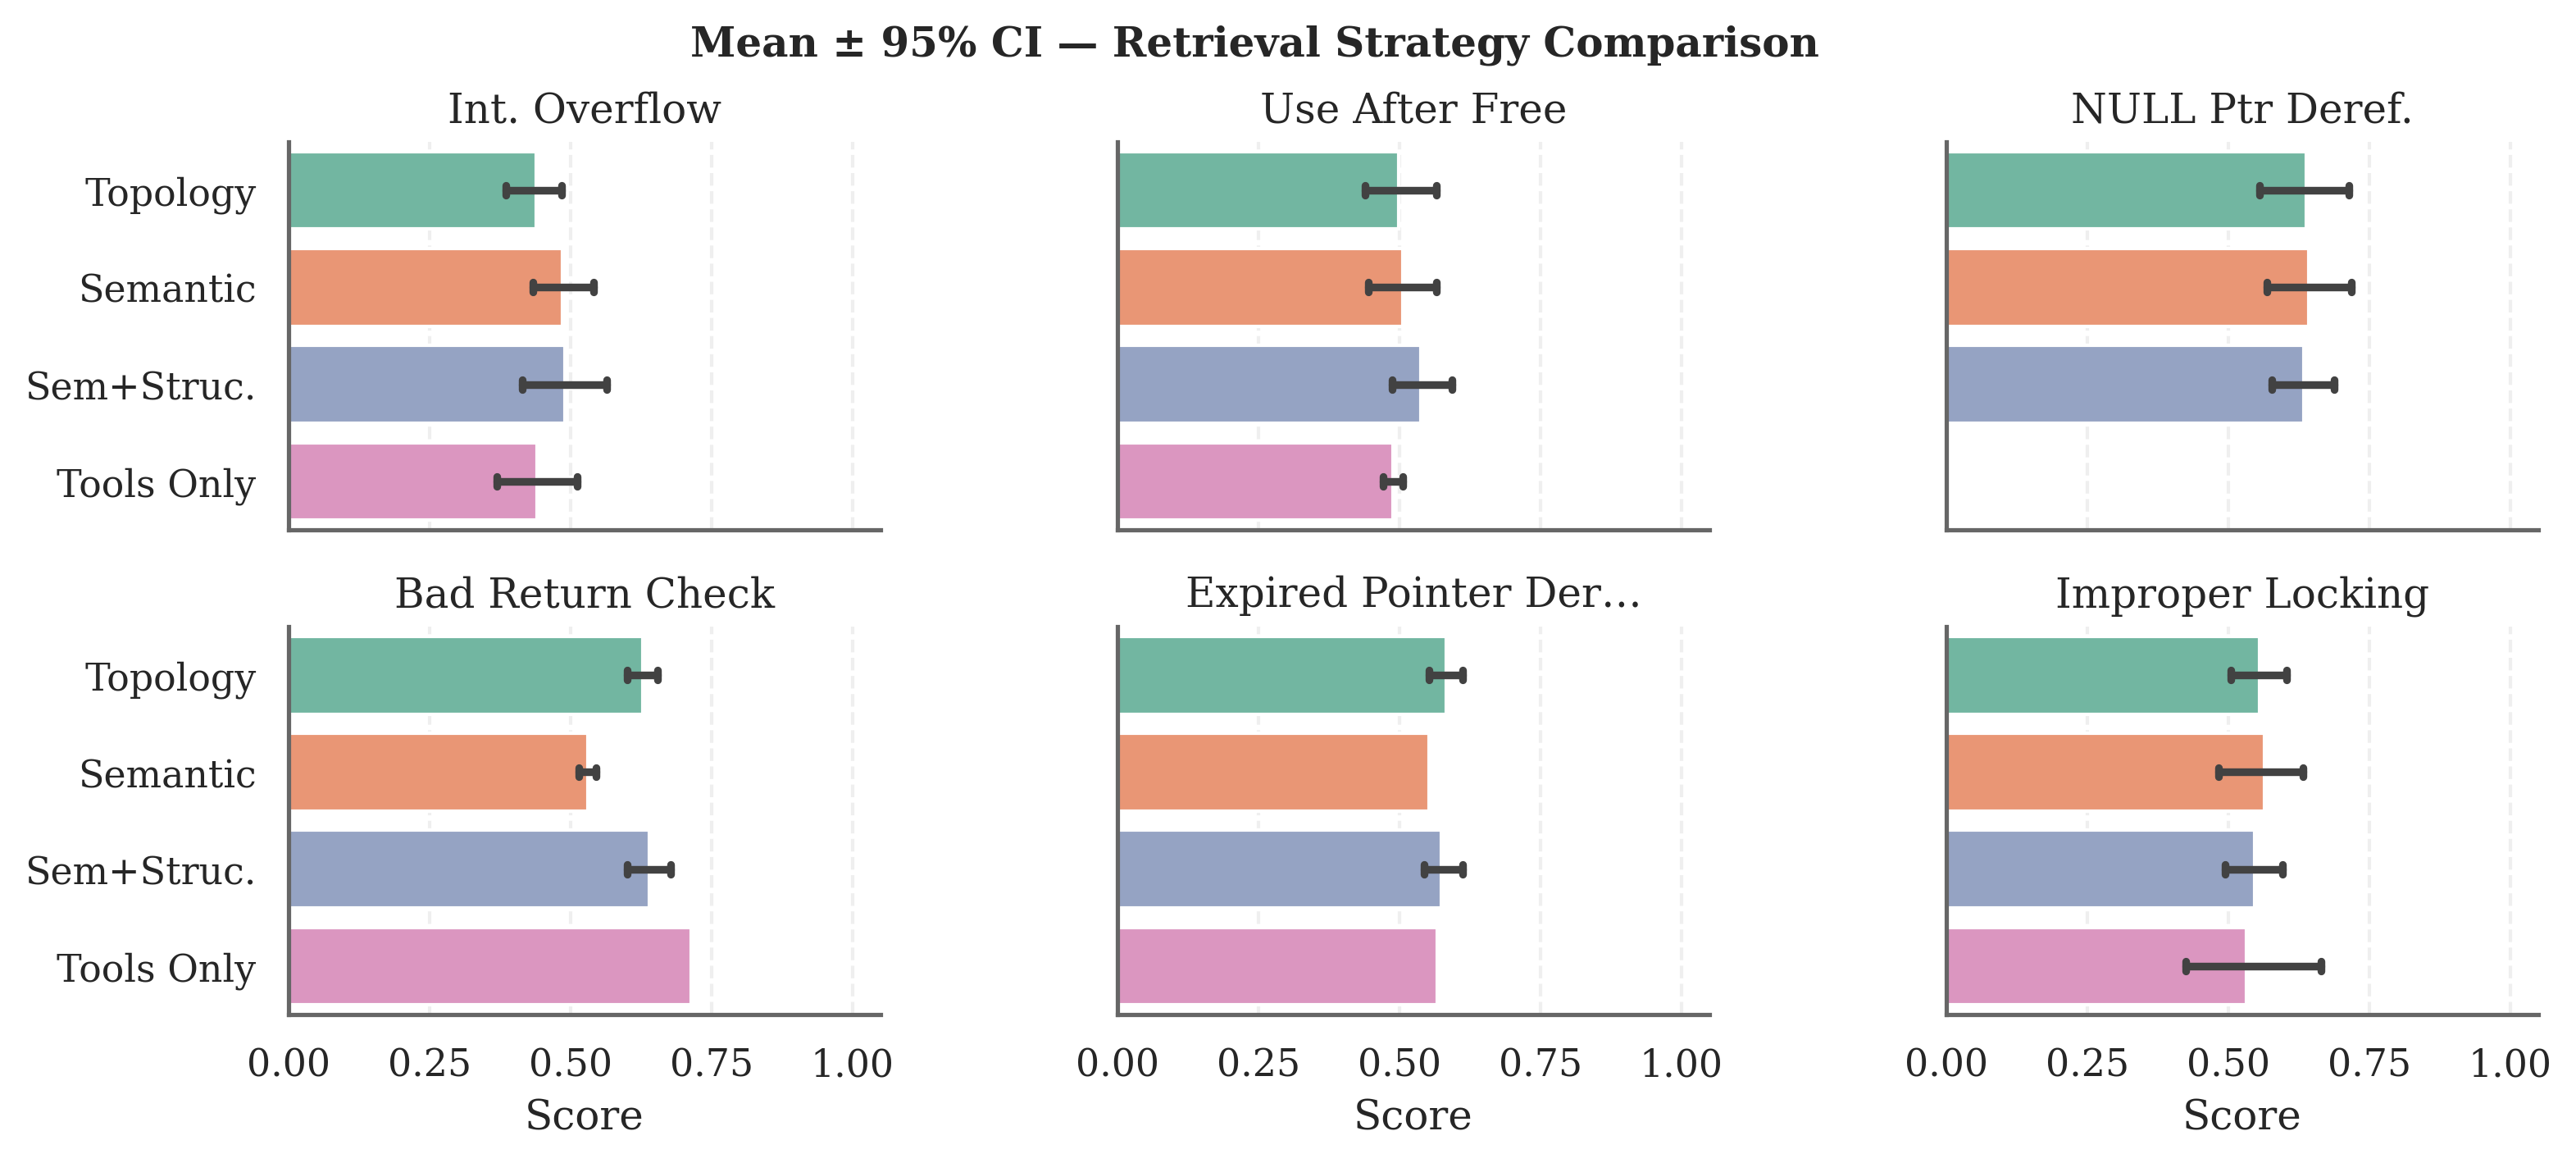
\includegraphics[width=1\linewidth]{img/patching/ci_gpt4_bertscore.png}
    \caption{BERTScore confidence intervals for GPT-4o patching on AutoPatch, grouped by CWE category.}
    \label{img:autopatch_gpt4o_bertscore}
\end{figure}
\begin{table}[H]
  \centering
  \caption{GPT-5.3-Codex: Overall pipeline performance on the autopatch dataset}
  \label{tab:autopatch_overall_pipeline_performance_gpt_codex}
  \begin{tabular}{lrrrrrr}
    \toprule
    Source & N & \makecell{Completion \\ \%} & BLEU-4 & BERTScore F1 & ROUGE-L F1 & \makecell{LLM\\ Judge\\ Valid} \\
    \midrule
    CodeBERT Pattern & 75 & 88.0 & 0.828 $\pm$ 0.000 & 0.525 $\pm$ 0.127 & 0.900 $\pm$ 0.106 & 70.3 \\
    CodeBERT Seq & 75 & 96.0 & 0.827 $\pm$ 0.000 & 0.527 $\pm$ 0.124 & 0.900 $\pm$ 0.100 & 82.7 \\
    Combined & 75 & 100.0 & 0.829 $\pm$ 0.000 & 0.521 $\pm$ 0.126 & 0.898 $\pm$ 0.100 & 85.3 \\
    \bottomrule
  \end{tabular}
\end{table}

\begin{table}[H]
  \centering
  \caption{GPT-5.3-Codex: Pipeline performance by CWE category on the autopatch dataset}
  \label{tab:autopatch_pipeline_by_cwe_category_gpt_codex}
  \begin{tabular}{llrrrr}
    \toprule
    Source & Category & N & BLEU-4 & BERTScore F1 & ROUGE-L F1 \\
    \midrule
    \multirow{4}{*}{CodeBERT Pattern} & Memory Safety & 22 & 0.842 & 0.539 & 0.917 \\\\
    & Concurrency & 28 & 0.799 & 0.518 & 0.867 \\
    & Numeric/Type & 10 & 0.865 & 0.314 & 0.911 \\
    & Resource Mgmt & 8 & 0.711 & 0.487 & 0.812 \\
    \midrule
    \multirow{4}{*}{CodeBERT Seq} & Memory Safety & 25 & 0.828 & 0.539 & 0.906 \\\\
    & Concurrency & 30 & 0.792 & 0.515 & 0.862 \\
    & Numeric/Type & 10 & 0.868 & 0.317 & 0.918 \\
    & Resource Mgmt & 7 & 0.743 & 0.515 & 0.831 \\
    \midrule
    \multirow{4}{*}{Combined} & Memory Safety & 26 & 0.830 & 0.537 & 0.902 \\\\
    & Concurrency & 31 & 0.804 & 0.514 & 0.873 \\
    & Numeric/Type & 11 & 0.889 & 0.315 & 0.931 \\
    & Resource Mgmt & 7 & 0.743 & 0.515 & 0.831 \\
    \midrule
    \bottomrule
  \end{tabular}
\end{table}

\appendix{}

\microtypesetup{protrusion=false}
\listoffigures{}
\listoftables{}
\microtypesetup{protrusion=true}
\printbibliography{}

\end{document}
